\chapter{Lattice gass cellular automata}
The first lattice gass cellular automaton was proposed in 1973 by Hardy, Pomeau and de Pazis, and it is called -- the HPP model.

Unfortunately, it could not do its job sufficiently well. For the reasons that we will sketch in this chapter, it does not converge to Navier-Stokes equations in macroscopic limit.

\bigskip

In the subsequent chapters we will explore two different approaches how to make functional LGCA. They both build on the idea of this imperfect HPP.

Therefore, we will explain the basic principles of HPP first, and later on, we will upgrade it - either to FHP, Pair-interaction or their multi-dimensional variants.

\section{From CA to LGCA}

The lattice of HPP is the simple rectangular 2D grid. At every point of a grid is a node, and this node is composed of 4 cells, see Figure~\ref{rectangular}.

\begin{figure}[htbp]
 \centering
 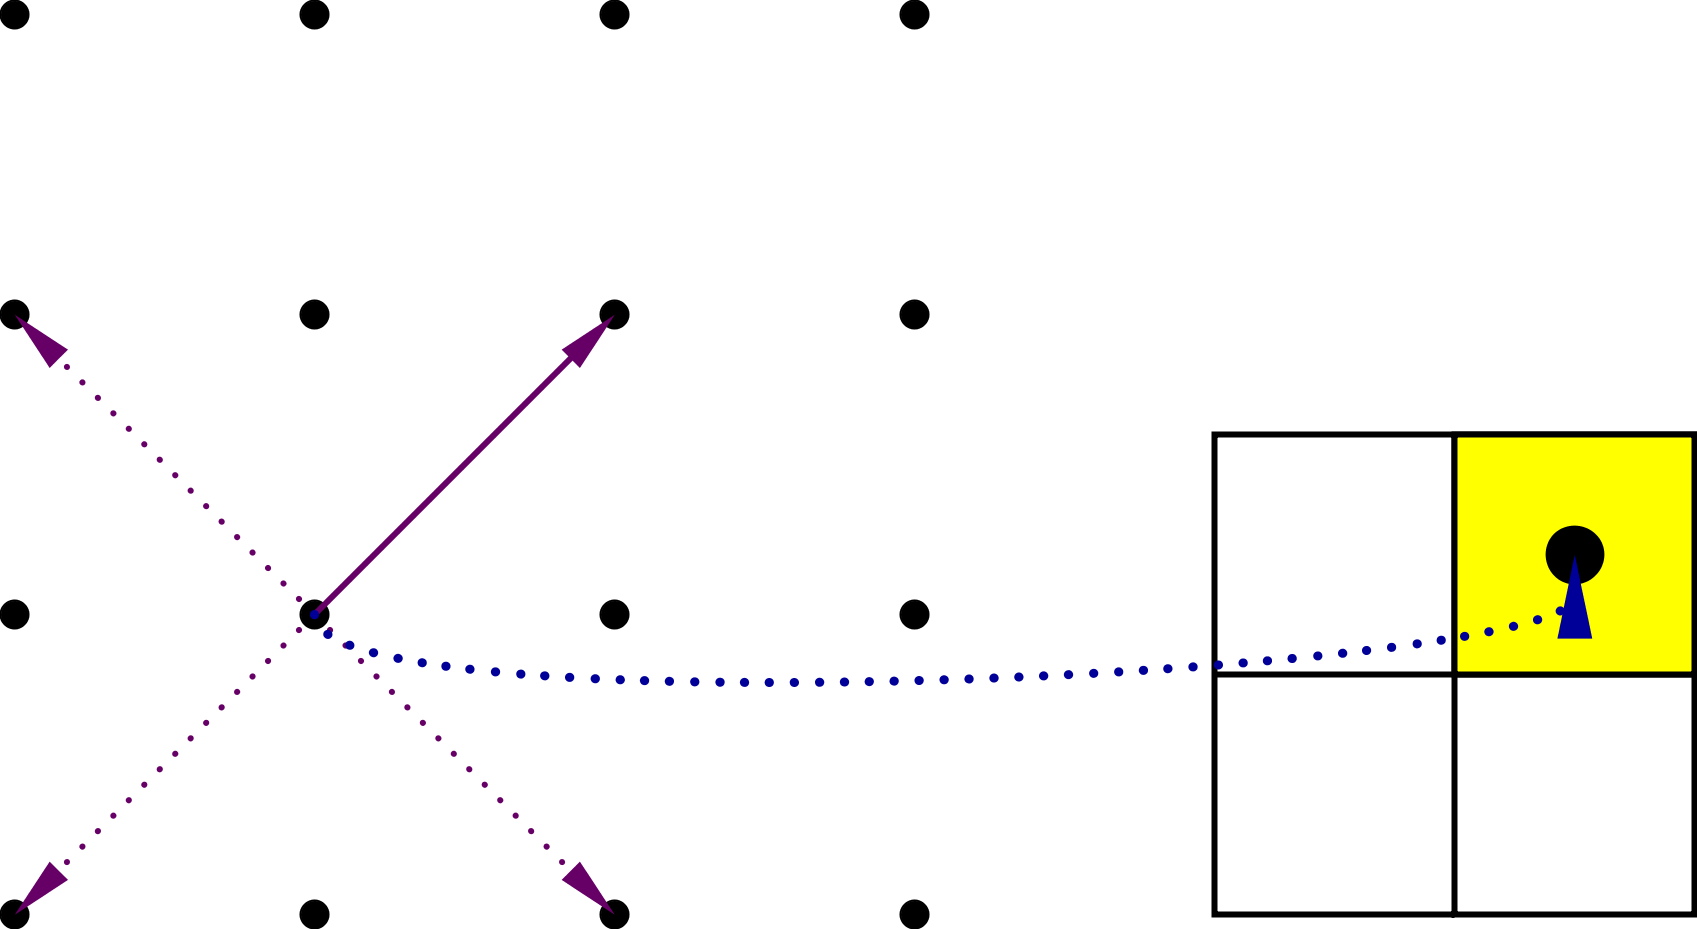
\includegraphics[width=0.6\textwidth]{./img/hppnode}
 \label{rectangular}
 \caption{Rectangular grid}
\end{figure}

Each of these cells can be in two states-- empty (white square) or occupied by the particle (yellow square).
The particle in this cell is heading to the diagonal node along the corresponding lattice vector.

\section{Update rule}
%The update rule should be design in such a manner, that is conserve physically relevant quantities, namely mass and momentum.

Every time-step, the position of the particles is changing. The update is done in two subsequent steps -- collision and propagation.

In the collision step, particles are swapped inside the single node, respecting two constraints - number of particle is same after the collision, and the total momentum in the node is same.

From these constraints follows that in HPP, there are only two collision configurations, see Figure~\ref{hpp-colision}.

\begin{figure}[H]
 \centering
 \includegraphics[width=0.7\textwidth]{./img/hpp_col}
 \label{hpp-colision}
 \caption{HPP colisions}
\end{figure}

These collision configurations are symmetric -- the first configuration is resolved to the other and vice versa.

If any other state gets changed, it would break the conservation of momentum and would be physically unrealistic.

\section{Propagation:}

After the collisions are resolved in every node, propagation follows -- figure \ref{hpp-prop}.
During propagation, particles move from node to node, along the lattice vectors that corresponds to the cells they occupied.
\begin{figure} [H]
 \centering
 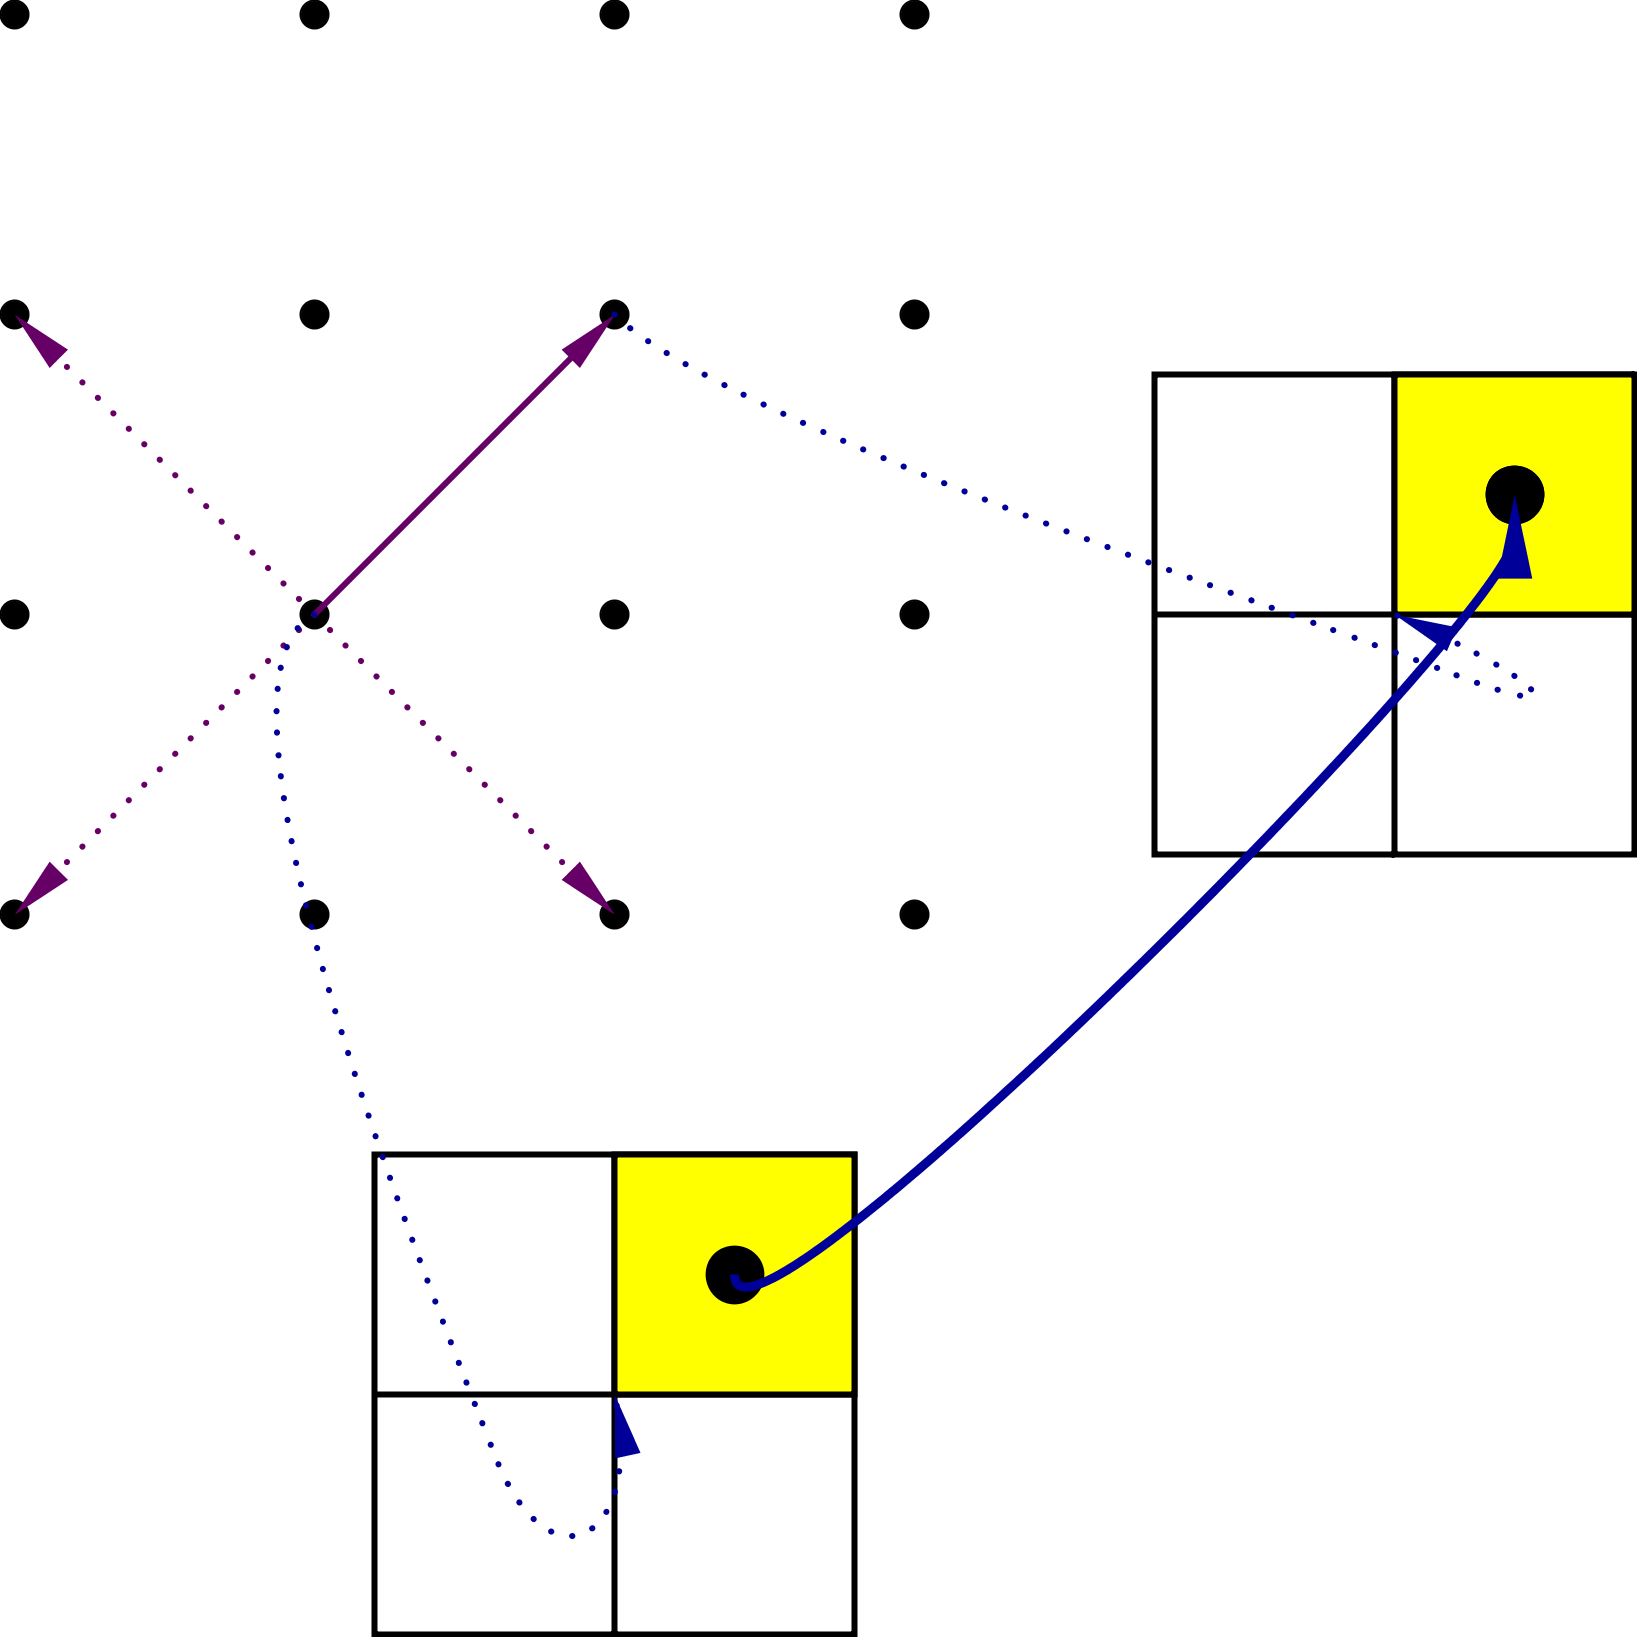
\includegraphics[width=0.6\textwidth]{./img/HPPprop}
 \label{hpp-prop}
 \caption{Propagation of particle from upper-left cell}
\end{figure}

\bigskip

\section{Conservation laws}

We already noted that collision and propagation conserve momentum, and they obviously conserve mass, since particles are neither created, nor anihilated during update. 
Let us inspect these conservation laws in the more depth by considering symmetries of this model.

Suppose we have lattice of infinite size (or finite size, but periodic boundary condition are used). Then if we shift the lattice by multiple of lattice vector, we get the same lattice -- the lattice is symmetric with respect to translation.
As we know by Norther's theorems, translational symmetry implies conservation of momentum.

\bigskip

Also, the grid possesses a rough rotational symmetry - rotation by the $90\degree$ leads to the same lattice.

However, this rectangular symmetry is not sufficient.
When we derive the hydrodynamic equations in the following chapter, we will observe that four lattice vectors lead to unrealistic equations, comparing to the models with six and more lattice vectors.

\bigskip
Another problem caused by low rotational symmetry are the non-physical quantities that are conserved nevertheless -- so called spurious invariants \footnote{The improved LGCA also posses the spurious \textit{Zanetti's invariants}, but they are under level of noise, due to higher symmetry or additional degrees of freedom in the node}.

Consider the total momentum in the node before and after collision on the figure \ref{hpp-colision}.
Let us decompose the total momentum into the cardinal directions:
\begin{align} 
P = P_N + P_S + P_E + P_W.
\end{align}
The total momentum $P$ is correctly conserved by HPP collison, but also quantities
\begin{align} \label{zanet}
P_{spur1} = P_N + P_E - P_S - P_W
\end{align}
and
\begin{align}
P_{spur2} = P_N + P_W - P_S - P_E
\end{align}
are conserved, although these quantities have no physical counterparts.

\bigskip


To conclude this chapter and finish-off the HPP, it is physically implausible because
\begin{enumerate}
\item angular momentum is not conserved due to insufficient rotational symmetry,
\item other non-physical quantities, so called \textit{spurious invariants} are conserved.
\end{enumerate}

Although it is a flawed model, it sparked interest of the wider community and various successful LGCAs evolved from HPP. In the next chapter, we will introduce the first successful branch of LGCAs -- the FHP model.